% $Id: PropagatorOverview.tex,v 1.1 2008/10/09 16:16:11 dconway Exp $
\chapter{\label{chapter:PropagatorOverview}Propagation in GMAT}
\chapauthor{Darrel J. Conway}{Thinking Systems, Inc.}

\section{Propagator Overview}

GMAT's model contains a subsystem that is used to move a user defined mission through time,
following the sequence of events defined in the Mission Control Sequence.  That subsystem is
referred to as the propagation subsystem.  In its most generic form, GMAT's propagation subsystem
can be thought of as taking a mission state $\textbf{X}_i$ at some time $t_i$ and moving that state
by some amount $\delta t$ to some new time $t_f$, resulting in a new state $\textbf{X}_f$.  The
components that are used to perform this change of state are the elements of the propagation
subsystem.  In other words, GMAT's propagation subsystem performs the actions needed to calculate
the new state by performing the operation

\begin{equation}\label{eq:abstractProp}
\textbf{X}_f(t_f) = F(\textbf{X}_i(t_i), \delta t)
\end{equation}

\noindent This chapter provides an overview of the definition of the quantities in this equation:
the definition of the mission state vector and all of its components, the evolution operator $F$
that moves the state vector, and an overview of the construction and decomposition of these
quantities in GMAT.

GMAT's propagation subsystem is used to perform all analytic propagation and numerical integration
needed by the system.  That includes modeling the time lines for spacecraft and formations, mass
depletion modeling during finite duration maneuvers, evolution of the state transition matrix,
attitude propagation, evolution of physical properties and their variances as needed for orbit and
attitude determination problems, and evolution of costate variables needed for optimal control
problems.  The diversity of propagation issues encountered in the coverage provided by the
propagation subsystem makes it a potentially quite complicated collection of components.  For that
reason, the subsystem is broken into a collection of different elements each tailored to specific
aspects of the propagation problem regime.  The propagation problem requires a consistent, complete
description of the evolution operators and the propagation vector, which are discussed briefly below
and in detail in Chapters~\ref{chapter:Propagators} and~\ref{chapter:PropagatorStates},
respectively.  This chapter concludes with a description of the scripting elements used to drive
propagation in GMAT, using the Propagate command as an example of this scripting.

\section{Propagator Overview}

The function $F$ in equation~\ref{eq:abstractProp} defines the process that takes a vector of
numbers defining system properties at one time and finds the values of those same properties at a
different time.  This process of moving the properties through time is performed using one
or more evolution operators.  The objects in GMAT that perform this evolution are the propagators.
GMAT's propagators are designed to support evolution either forwards or backwards in time.  The
propagators can be set to run in a synchronized manner or independently of one another.  The
selection of the category and type of propagator that is used is selected by the user based on the
types of parameters that need to be propagated.

GMAT Supports three different categories of propagators, defined by the type of data available for
the propagation.  The categories are

\begin{description}
\item[Analytic] GMAT's analytic propagators take a known, closed form solution to the evolution
problem and apply that solution to the propagation vector specified at some initial time to find its
values at some other time.  GMAT's analytic propagators use embedded evolution equations to
calculate the values of parameters at the desired times.
\item[Numerical] The numerical propagators find a solution of the differential equations of motion
for the parameters using a precision numerical integrator and derivative models.  Propagators in
this category consist of a pair of objects: a numerical integrator derived from the Integrator class
and a derivative model derived from the PhysicalModel class.
\item[Precalculated]  Precalculated parameter values are retrieved -- and, if needed, interpolated
-- from files containing the time history of the parameter values.
 \end{description}

Each category of propagator supplies implementations of core methods designed to standardize
the propagation interface.  The core propagation interfaces are defined in the Propagator base
class.  Every GMAT propagator uses these interfaces to perform the following actions:

\begin{itemize}
\item Map the propagation vector to known evolution operators
\item Initialize all data structures and object references needed to propagate
\item Load the initialized data structure immediately before propagating
\item Propagate the propagation vector
\item Reset the propagator to use its initial settings
\end{itemize}

\noindent The Propagator class defines these interfaces to perform the actions listed above:

\begin{description}
\item[GetPropagatorOrder]  GMAT includes both first and second order numerical integrators.  This
interface is used to determine which is needed for a particular integrator.  The non-numerical
integrators all report order 0.
\item[SetPhysicalModel]  The SetPhysicalModel method sets the derivative model used for numerical
integration, and -- for all propagators -- performs pre-initialization tasks required before
initialization can proceed.  This method ensures that all of the elements needed for evolution have
been set for the propagator.
\item[Initialize]  All of the reference object pointers and other interconnections necessary for
propagation are set in the Initialize method.  Propagators that do not allow for dynamic resizing of
the propagation vector also use this method to initialize the propagation vector mapping needed for
the evolution.  Those that may require dynamic resizing perform a preliminary mapping during
initialization.
\item[Update]  The Update method is used to reset the propagator when the underlying physical model
changes.  This method is used to refresh the propagation vector mapping if the propagation vector
has changed -- for instance, when a transient derivative is applied or removed to model mass flow
during a finite maneuver.  It also resets some of the propagator's properties if needed, like the
initial step size for variable step propagators.
\item[ResetInitialData]  The ResetInitialData method sets a flag telling the propagator that at the
next call to propagate the propagation vector, the propagator's initial data needs to be updated
prior to propagation.
\item[Step]  State evolution is driven through calls to the Step method.  Different categories and
subcategories of propagators implement different versions of this method based on the needs and
capabilities of the propagators.
\end{description}

\noindent These methods define the minimum level of interface required for every GMAT propagator.
The Propagator subclasses extend this set based on the needs of the category of the propagator
defined in the subclass.

The design details for the propagators are provided in Chapter~\ref{chapter:Propagators}.

\section{Propagation Vector Overview}

The propagators evolve a vector of data from one epoch to another.  The data that evolves is
contained in a column vector sized to match the evolving data.  This vector is assembled and
populated prior to propagation based on specifications scripted by the user.  The propagation
vector provides methods that support the following actions:

\begin{itemize}
\item Supply epoch information
\item Supply propagation vector information, including all of the following:
\begin{itemize}
\item Size of the vector
\item Element by element types for mapping the vector onto the propagator
\end{itemize}
\item Supply the propagation vector
\end{itemize}

\noindent GMAT uses a class, PropVector, to model the propagation vector.  The PropVector objects
supply the information used to assemble the derivative vector needed for numerical integration, the
epoch and state data needed for analytic propagation, or the epoch and time step information used
for precalculated propagation.

The PropVector class defines these interfaces to perform the actions listed above:

\begin{description}
\item[GetEpoch and SetEpoch]  A PropVector contains data calculated at a single epoch.  These
GetEpoch and SetEpoch methods provide access to the epoch data in the PropVector.
\item[GetDimension]  Retrieves the current size of the PropVector -- that is, the number of
elements that evolve over time.  The dimension is used to initialize the propagator, and, in
conjuction with the vector map, to ensure that the correct operator is used to evolve each element
of the vector.
\item[GetVectorMap]  Retrieves the mapping of the PropVector, element by element, so that the
evolution components can be set correctly.
\item[GetVector]  Retireves a pointer to the Real array of data for the vector.  The retrieved
vector has the size given by the dimension of the PropVector, mapped as specified in the vector
map.  Components that use the PropVector for propagation can both read and write to this retrieved
vector.  This violation of encapsulation is intentional, in order to make the propagation process
as fast as possible in GMAT.
\end{description}

\noindent These interfaces define the minimal interfaces necessary for PropVector objects.  They
are defined as overridable interfaces so that classes can be derived form PropVector in the future
as needed.

The PropVector class is managed through a mapping class, the MissionState.  The MissionState class
is a container class -- it contains references to the objects providing state data that evolves
using GMAT's evolution operators, as defined in its Propagator classes.  The MissionState class
provides methods accessed by the propagators to construct, retrieve, and update the PropVector.  It
manages the data flow between these objects and the propagation vectors manipulated by the
Propagators.  The MissionState builds the PropVectors used by the propagators, setting up the data
vector and associated component mappings used by the propagator to assemble the elements needed for
propagation.

The MissionState class defines a set of interfaces used to manage the data soureces used to assemble
the PropVector.  The interfaces supplied by the MissionState for these tasks are:

\begin{description}
\item[AddObject]  Adds an object that supplied data to one or more PropVectors.
\item[Initialize]  Constructs the PropVector or PropVectors used by a propagator.
\item[PrepareToPropagate] Completes PropVector initialization needed prior to propagation.
\item[GetPropVector]  Retrieves an assembled PropVector designed for propagation.
\end{description}

\noindent Each one of GMAT's propagators uses a MissionState object to manage the data that is
propagated.

The PropVector and MissionState classes are described in detail in
Chapter~\ref{chapter:PropagatorStates}.

\section{Scripting Propagation}

As is described above, GMAT provides three approaches to propagation.  The system can model the
evolution of the state data by numerically integrating the equations of motion, providing a high
precision model of the evolution, by reading the data from a pre-calculated file of data points
(e.g. a SPICE file), or by using an analytical propagator that provides a fast, lower fidelity
vector of propagated data.  The propagation subsystem can perform these tasks for all of the
parameters represented in the propagation vector: for the spacecraft orbit and attitude data, mass
properties, for the state transition matrix and covariance matrices, and for any other parameters
placed in the propagation vector, as long as the underlying propagation model supporting the
parameter exists.  For the numerical integrators, that means that the  set of ordinary differential
equations describing the evolution have been coded into the system.  Similarly, analytic
propagators require encoding of the analytic equations of motion.  The precalculated data
propagators require an ephemeris or similar time based file of the evolution of the paramteres that
they propagate.  GMAT is designed to support mixed mode propagation as well; elements propagated in
a Mission Control Sequence command need not all be propagated using the same approach.  Some can be
propagated analytically or using a file while others are numerically integrated.  The design
implementing this mode is described in Chapter~\ref{chapter:Propagators} and in the descriptions of
the commands that support propagation.

Commands that drive propagation follow the process shown in
Figure~\ref{figure:CommandPropagationOverview}.  The command is initialized in the Sandbox along
with the rest of the Mission Control Sequence.  During this initialization, specific pieces
required to initialize each propagator driven by that command are performed.  There are portions of
the propagation process that cannot be initialized at this point in the mission run because they
depend on data that may be changed when commands that precede the one invoking propagation fire.
This final piece of initialization is performed in a method named PrepareToPropagate(), which is
called when the command's Execute() method is called, immediately before the actual propagation.
Finally, the propagation is performed in the body of the Execute() method associated with the
command.

\begin{figure}[htb]
\begin{center}
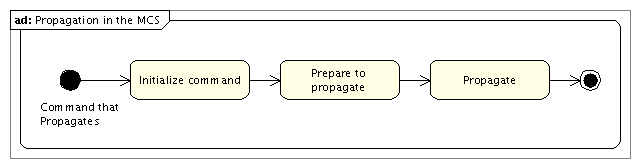
\includegraphics[320,84]{Images/PropagationintheMCS.png}
\caption[Command and Propagation Processes]{\label{figure:CommandPropagationOverview}Command and
Propagation Processes}
\end{center}
\end{figure}

\subsection{Example: The Propagate Command}

Propagation is scripted in GMAT through the creation of propagator objects and the incorporation of
these objects into the Mission Control Sequence through propagator enabled commands.  The
prototypical propagator enabled command is the Propagate command (described more fully in
Section~\ref{section:Propagate}), scripted in its simplest form like this:

\begin{quote}
\begin{verbatim}
Propagate prop(sat)
\end{verbatim}
\end{quote}

\noindent The command shown here consists of three elements: the Propagate keyword, the name of the
propagator that is used (``prop'' in this case), and the object that is propagated, ``sat'' in
this example.  In order for this command to run, the objects used in teh propagation must exist, so
there must be matching creation commands.  Assuming that the command exists in the main script
rather than a function, that means these lines must occur before the Propagate command line:

\begin{quote}
\begin{verbatim}
Create Spacecraft sat;
Create Propagator prop;
\end{verbatim}
\end{quote}

\noindent The propagated object can, of course, be any object that supplies a propagation vector for
propagation.

The type of propagator is specified by setting the ``Type'' property on the propagator object, like
this:
\begin{quote}
\begin{verbatim}
prop.Type = PrinceDormand78;  % Use a Prince-Dormand RK integrator
\end{verbatim}
\end{quote}

\noindent The Type setting for the propagator must be made before setting any other propagator
properties because the properties for the propagator depend on the type of Propagator object that is
being used.  Every GMAT propagator has default values for each of its properties.  Users override
these settings to tailor the behavior of the propagator.

The following sections describe the scripting for each category of Propagator.

\subsubsection{Scripting Numerical Integrators}

The numerical integrators require an additional object defining the forces and other differential
equations that are used to model the propagation.  These pieces are gathered in a container class,
the ODEModel class derived from PhysicalModel.  The ODEModel class plays several roles in the
propagation subsystem:

\begin{itemize}
\item It works with a MissionState object to create the propagation vector
\item It coordinates the data mapping between the objects that are propagated and the propagation
vector
\item It handles the superposition tasks when the differential equations defining propagation
consist of multiple components
\end{itemize}

\noindent The ODEModel class is described more fully in Section~\ref{section:TheODEModel}.
Scripting for ODEModel objects depends on context.  For orbit propagation, the ODEModel is scripted
as a ForceModel component, using this syntax:

\begin{quote}
\begin{verbatim}
Create ForceModel forces;
forces.CentralBody = Earth;
forces.PrimaryBodies = {Earth};
forces.Drag = MSISE90;
forces.SRP = On;
forces.ErrorControl = RSSStep;
forces.GravityField.Earth.Degree = 4;
forces.GravityField.Earth.Order = 4;
forces.GravityField.Earth.PotentialFile = 'JGM2.cof';
forces.PointMasses = {Sun, Luna, Mercury, Venus, Mars};

Create Propagator prop;
prop.Type = PrinceDormand78;
prop.FM = forces;
\end{verbatim}
\end{quote}

\noindent The forces that are included in the differential equations of motion are defined by
specifying the desired elements and, when needed, properties of those elements.  The resulting
ODEModel is assigned to the integrator by assigning its name to the FM property of the Propagator.

\subsubsection{Scripting Analytic Propagators}

This section is TBD, based on requirements and design for analytic propagators when they are added
to GMAT.

\subsubsection{Scripting Precalculated Propagators}

\textit{Detailed information for this section is TBD, based on requirements and design for the SPICE
file component and discussions of other ephemeris based propagators planned for GMAT.  However, the
scripting discussion is underway, and included here, subject to extensive revision.}

Propagation based on precalculated data is used in GMAT to propagate data for spacecraft, celestial
bodies not modeled elsewhere, and other elements that are described using file-based time-indexed
data.

Scripting for the precalculated propagators is similar to that for the numerical integrators.  The
precalculated propagators identify the propagator type as one of the supported file based propagator
types, and identify a file -- the file containing the ephemeris data -- rather than a force model.
An example of the setup for a SPICE file based precalculated propagator for the Clementine mission
is given here:

\begin{quote}
\begin{verbatim}
Create Spacecraft Clementine
Clementine.EphemID = -40      % Clementine's NAIF ID

Create Asteroid Geographos    % Asteroid support is a future enhancement;
                              % use a Spacecraft with the current code base
Geographos.EphemID = 2006513  % No clue about the real NAIF ID for Geographos...

Create Propagator prop
prop.type = SPICE
prop.StepSize = 300    % seconds
prop.Ephemeris = DSPSE.SPK        % Ephem containing Clementine and Geographos
prop.Ephemeris = SolarBodies.SPK  % Second ephem used to add vectors together
\end{verbatim}
\end{quote}

\noindent Propagation with a SPICE file propagator is handled identically to that performed using
other propagators.  For the asteroid encounter phase of the mission above, a user could script the
propagaton like this:

\begin{quote}
\begin{verbatim}
Create Variable i
For i = 0 : 2000
   Propagate prop(Clementine, Geographos)
EndFor
\end{verbatim}
\end{quote}

\noindent One constraint imposed in GMAT is that for a single ephemeris based propagator, each
object that is propagated must be contained in the same ephemeris file.  That means that in the
example above, the ephemeris for both the Clementine spacecraft and the asteroid Geographos must
exist in the SPICE file DSPSE.SPK.  For this case, the same result could be achieved with separate
ephemerides for the spacecraft and asteroid with this scripting:

\begin{quote}
\begin{verbatim}
Create Spacecraft Clementine
Clementine.EphemID = -40   % Clementine's NAIF ID

Create Asteroid Geographos    % Asteroid support is a future enhancement;
                              % use a Spacecraft with the current code base
Geographos.EphemID = 2006513  % No clue about the real NAIF ID for Geographos...

Create Propagator prop
prop.type = SPICE
prop.StepSize = 300    % seconds
prop.Ephemeris = Clementine.SPK   % Ephem containing Clementine
prop.Ephemeris = SolarBodies.SPK  % Second ephem used to add vectors together

Create Propagator geogProp
geogProp.type = SPICE
geogProp.StepSize = 300    % seconds
geogProp.Ephemeris = Asteroids.SPK    % Ephem containing Geographos
geogProp.Ephemeris = SolarBodies.SPK  % Second ephem used to add vectors together

Create Variable i
For i = 0 : 2000
   Propagate Synchronized prop(Clementine) geogProp(Geographos)
EndFor
\end{verbatim}
\end{quote}

\noindent Finally, you may have noted that a second ephemeris source is identified for the SPICE
propagator.  This option is scripted in these examples to allow conversion of the epheris data for
propagated objects to other bodies in the model.  For example, the ephemeris for Geographos is
likely to be calculated with respect to the Sun.  GMAT may need Earth-centered states, so the SPICE
propagator needs to load the SPICE kernel that describes the Earth's location with respect to the
Sun in order to add the position vectors together to build the state vector.

The following chapters provide details of the propagation subsystem components.
Chapter~\ref{chapter:PropagatorStates} describes the PropVector and MissionState classes, and
includes descriptions of the data mapping for vector elements and diagrams describing hte layout of
the PropVector data for single and multiple objects.  Chapter~\ref{chapter:Propagators} describes
the design of the propagator classes.  The commands that control the propagation subsystem are
described in Chapters~\ref{chapter:Commands} and~\ref{chapter:SpecificCommands}.


% \subsection{The Equations of Motion}
%
% \subsection{Division of Labor: Integrators and Forces}
%
% \section{Integrators}
%
% \section{\label{section:ForceModelOverview}The GMAT Force Model}
%
% \subsection{The PhysicalModel Class}
%
% \subsection{The ForceModel Class}
%
% \subsubsection{Adding and Removing Forces}
%
% \subsection{Applying Forces to Spacecraft}
%
% \section{The State Vector}
%
\section{\label{section:PropagationExample}Example: Propagation of Two Spacecraft}

In this section, the object creation and interactions will be examined in some detail for the
following script:

\begin{quote}
\texttt{Create Spacecraft sat1 sat2\\
sat1.TA = 90.0;\\
sat2.TA = 91.0;\\
\\
Create ForceModel fm\\
fm.CentralBody = Earth\\
fm.PrimaryBodies = \{Earth\}\\
fm.Drag = MSISE90\\
fm.SRP = On\\
fm.GravityField.Earth.Degree = 4\\
fm.GravityField.Earth.Order = 4\\
fm.PointMasses = \{Sun, Luna\}\\
\\
Create Propagator prop\\
prop.FM = fm\\
prop.Type = PrinceDormand78\\
prop.InitialStepSize = 60\\
prop.Accuracy = 1.0e-12\\
prop.MinStep = 1.0e-6\\
prop.MaxStep = 2700.0\\
prop.MaxStepAttempts = 50\\
\\
Propagate prop(sat1, sat2) \{sat1.ElapsedDays = 1.0\}}
\end{quote}

GMAT collects the integrator and force model in a container called a PropSetup.  GMAT's PropSetup
class has a member pointer for a Propagator and a second pointer for an ODEModel.  Each PropSetup
also has a StateManager member -- in the case of propagation, the StateManager is an instance of the
PropagationStateManager class -- that communicates with the other objects in the system to retrieve
the values of the data that needs to be propagated and arranges those data into a single vector that
the force model and integrator understand. GMAT's propagation subsystem -- that is, the integrator
and associated ODEModel -- use this data vector and an associated mapping of ordinary differential
equations to calculate a new vector of numbers at some different time.  In other words, GMAT's
propagation subsystem has minimal knowledge of the objects that are being propagated.  At the level
of the evolution algorithm, the propagation subsystem merely maps a vector of numbers at some epoch
into a new vector of number at some other epoch.  The propagation state manager associated with the
PropSetup container handles the communications of that vector numbers with the corresponding data in
the objects.

Returning to our example, when the scripting listed above is built, GMAT constructs two spacecraft
named sat1 and sat2.  These spacecraft are added to GMAT's configuration.  Next GMAT creates an
ODEModel named fm and adds it to the configuration.  Then GMAT creates a PropSetup named prop and
 adds it to the configuration\footnote{The command ``Create Propagator prop'' uses GMAT's factories
to build a PropSetup container named prop.}.  The PropSetup, prop, includes a member instance of the
PropagationStateManager class, and two pointers: a pointer to a Propagator object and a pointer to
an ODEModel object, both initialized to NULL.  The object configuration lines, omitted in this
example, populate the Propagator side of that PropSetup.  Finally, the line ``prop.FM = fm''
assigns the ODEModel named fm to the PropSetup.  This object creation and configuration is stored
in GMAT's configuration for use during a run.

The Propagate command is treated similarly.  An instance of the Propagate command is created using
GMAT's factory subsystem and then placed in the Mission Control Sequence.  The command is passed
the string that was used to construct it, and that string is decomposed into its constituent
elements.  Once that phase is complete, the Propagate command has strings defining the PropSetup
used for propagation, the names of the objects that need to be propagated, and strings defining the
condition or conditions that terminate propagation.  In our example, the Propagate instance has a
single string defining the PropSetup it uses, ``prop'', a StringArray defining the objects that are
propagated using that PropSetup -- ``sat1'' and ``sat2'' -- and strings identifying the object used
to determine when to stop -- ``sat1'' -- the type of condition that terminates propagation --
``ElapsedDays'' -- and the value that that condition should have when it propagation ends
--~``1.0''.

\begin{table}
\begin{center}
% use packages: array
\begin{tabular}{llll}
Object & Elements & References & Comments \\
sat1 & state vector & none &  \\
sat2 & state vector & none &  \\
fm &  & member forces &  \\
prop & psm 'fm' ['sat1' 'sat2'] & Integrator &  \\
prop.psm &  &  &
\end{tabular}
\caption[Parameter Configuration after Parsing]{Parameter Configuration for Objects Created after
Script Parsing}
\end{center}
\end{table}
